\chapter{Requirements}
\section{Allgemeine Beschreibung}
\subsection{Produktperspektive}
Mit Internet of Things sind eine Vielzahl neuartiger Devices entstanden. Während in herkömmlichen Netzwerken hauptsächlich Personal Computer, Notebooks, Server usw. verwaltet werden mussten, so bringen IoT Devices den IT-Abteilungen neue Herausforderungen. Zum einen dürfte die Anzahl Geräte gegenüber herkömmlichen Computer deutlich ansteigen, zum anderen sind IoT Devices in Sachen Funktionalität und Rechenleistung, sowie auch der Netzwerkbandbreite deutlich beschränkt. 

Mit diesem Projekt soll ein Prototyp einer Management Applikation bereitgestellt werden, um eine grosse Anzahl unterschiedlicher IoT Devices administrieren zu können. 
\subsection{Produktfunktionen}
Die Applikation soll den Benutzern erlauben, IoT Geräte zu verwalten. Die Aufgaben reichen vom Discovery von Devices über die Konfigurationsverwaltung und Softwareverteilung bis zu Backup und Restore. Ausserdem sollen Management-relevante Kommandos auf Devices ausgeführt- und Security Aspekte beachtet werden. Die Details zu den Produktfunktionen sind den Use Cases zu entnehmen.

\subsection{Benutzer Charakteristik}
Zielpersonen der Applikation sind Betreiber von IoT Devices. Dies können im Enterprise Umfeld IT-Mitarbeiter in operationeller Funktion-, oder auch Softwareentwickler für IoT Applikationen sein. Heimanwender können bei entsprechenden Kenntnissen ebenfalls zur Zielgruppe gehören. Es werden solide Grundkenntnisse in TCP/IP Netzwerken sowie Verständnis der verwendeten IoT Architekturen und Devices vorausgesetzt. Es werden ausserdem Grundkenntnisse des LwM2M Protokolls empfohlen. 
\section{Use Cases}
\label{sec:usecases}
\subsection{Use Cases Diagramm}
\begin{figure}[H]
\centering
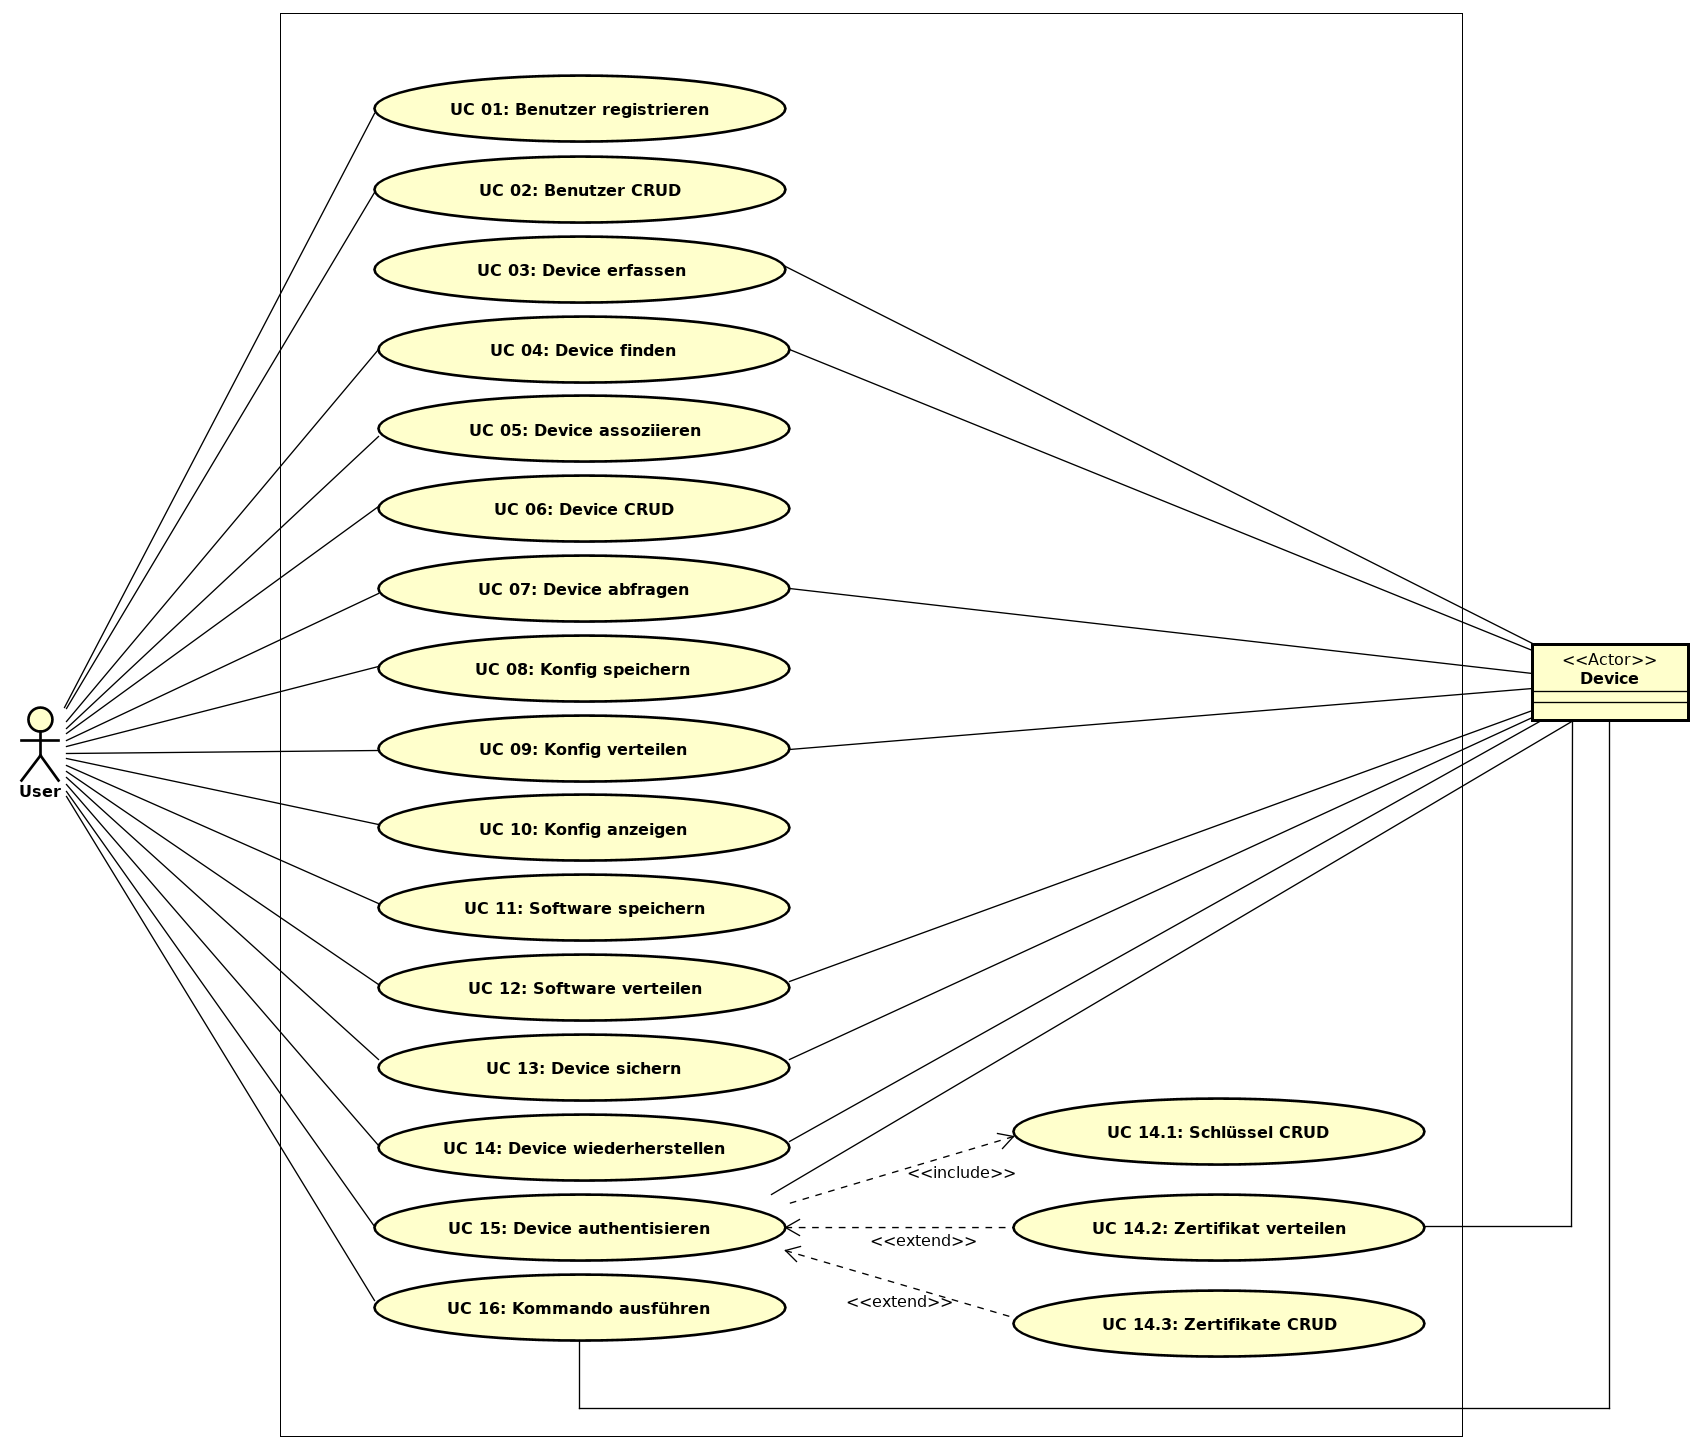
\includegraphics[scale=0.42]{../02_Analyse/images/use_case_diagram.png}\caption{Use Case Diagramm}
\end{figure}

\subsection{Aktoren}
Der Benutzer der Applikation ist in diesem System der einzige primäre Aktor. Dieser bewirtschaftet die Applikation und verwaltet alle Devices und Benutzer. Als Sekundärer Aktor werden die einzelnen Devices gezählt.
\newpage
\subsection{Beschreibungen (Casual)}
\subsubsection{Login User}
\mbox{}
\begin{longtable}{| p{4cm} | p{11.7cm} |}
 \hline
 \textbf{ID} & 01\\ \hline 
 \textbf{Name} & Login User\\ \hline 
 \textbf{Beschreibung} & Der Benutzer loggt sich in die Applikation ein.\\ \hline 
 \textbf{Preconditions} & 
   \tabitem Applikation gestartet \newline
   \tabitem Benutzer im System angelegt
  \\ \hline 
 \textbf{Postconditions} & 
  \tabitem Benutzer kann auf dem Management Startseite interagieren.
 \\ \hline
 \textbf{Main Success Scenario} &
 1. Loginseite erscheint beim Start der Applikation \newline
 2. Benutzer gibt Benutzername und Passwort ein \newline
 3. Benutzer wählt \glqq Login\grqq . \newline
 4. Benutzer ist eingeloggt.
\\  \hline 
 \textbf{Extensions} & 
 4.a Fehlermeldung bei falschem Login erscheint.   
 \\ \hline 
 \end{longtable}

\subsubsection{User CRUD}
\mbox{}
\begin{longtable}{| p{4cm} | p{11.7cm} |}
 \hline
 \textbf{ID} & 02\\ \hline 
 \textbf{Name} & User CRUD\\ \hline 
 \textbf{Beschreibung} & Benutzerverwaltung der Applikation\\ \hline 
 \textbf{Preconditions} & 
   \tabitem Applikation gestartet \newline
   \tabitem Benutzer ist registriert \newline
   \tabitem Benutzer ist eingeloggt 
  \\ \hline 
 \textbf{Postconditions} & 
  \tabitem Änderungen gespeichert
 \\ \hline
 \textbf{Main Success Scenario} &
 \textbf{Create:}\newline
  1. UC 01: Benutzer registrieren \newline
 \textbf{Read:}\newline
  1. Benutzer lässt Userdaten anzeigen \newline
 \textbf{Update:}\newline
  1. Benutzer lässt Userdaten anzeigen \newline
  2. Benutzer verändert Attribute\newline
  3. Benutzer speichert Änderungen\newline
 \textbf{Delete:}\newline
  1. Benutzer wird gelöscht \\ 
 \hline 
 \textbf{Extensions} & -\\ \hline 
 \end{longtable}

\subsubsection{Group CRUD}
\mbox{}
\begin{longtable}{| p{4cm} | p{11.7cm} |}
 \hline
 \textbf{ID} & 03\\ \hline 
 \textbf{Name} & Group CRUD\\ \hline 
 \textbf{Beschreibung} & Gruppenverwaltung der Applikation
 \\ \hline 
 \textbf{Preconditions} & 
   \tabitem Applikation gestartet \newline
   \tabitem Benutzer eingeloggt
  \\ \hline 
 \textbf{Postconditions} & 
  \tabitem Falls ein Gerät gefunden wird, wird es angezeigt 
  \\ \hline 
 \textbf{Main Success Scenario} & 
  \textbf{Create:}\newline
  1. Benutzer wählt ''Add New Group''. \newline
  2. Benutzer erfasst Name für Gruppe. \newline
 \textbf{Read:}\newline
  1. Benutzer navigiert zur Gruppennavigation.\newline
  2. Benutzer wählt eine Gruppe zur Anzeige aus \newline
  2. Gruppendetails werden angezeigt \newline
 \textbf{Update:}\newline
  1. Benutzer navigiert zur Gruppennavigation.\newline
  2. Benutzer passt Gruppeninformationen an. \newline
 \textbf{Delete:}\newline
1. Benutzer navigiert zur Gruppennavigation.\newline
  2. Benutzer wählt ''Delete Group''. \newline
  3. Gruppe wird vom System gelöscht.
  \\ \hline 
 \textbf{Extensions} & 
  -
  \\ \hline 
\end{longtable}


\subsubsection{Device CRUD}
\mbox{}
\begin{longtable}{| p{4cm} | p{11.7cm} |}
 \hline
 \textbf{ID} & 04\\ \hline 
 \textbf{Name} & Device erfassen \\ \hline 
 \textbf{Beschreibung} & Der Benutzer möchte ein Device hinzufügen. 
 \\ \hline 
 \textbf{Preconditions} & 
   \tabitem Applikation gestartet \newline
   \tabitem Benutzer eingeloggt \newline
   \tabitem Device ist registriert (UC06)
  \\ \hline 
 \textbf{Postconditions} & 
  \tabitem Device in Datenbank gespeichert (Attribut added = true)
  \\ \hline 
 \textbf{Main Success Scenario} & 
  \textbf{Create:}\newline
  1. UC 06: Discover Device
 \textbf{Read:}\newline
  1. Benutzer navigiert zur Geräteübersicht \newline
  2. Device details werden angezeigt \newline
  3. Benutzer wählt Objekt und klickt ''Read''.
 \textbf{Update:}\newline
  1. Benutzer navigiert zur Geräteübersicht \newline
  2. Benutzer passt Geräteinformationen an. \newline
 \textbf{Delete:}\newline
  1. Benutzer navigiert zur Geräteübersicht \newline
  2. Benutzer wählt \glqq delete\grqq . \newline
  3. Gerät wird vom System gelöscht.
  \\ \hline 
 \textbf{Extensions} & 
	-
  \\ \hline 
\end{longtable}

\subsubsection{Manage Components Hierarchy}
\mbox{}
\begin{longtable}{| p{4cm} | p{11.7cm} |}
 \hline
 \textbf{ID} & 05\\ \hline 
 \textbf{Name} & Manage Components Hierarchy\\ \hline 
 \textbf{Beschreibung} & Gruppenhierarchie verwalten\\ \hline 
 \textbf{Preconditions} & 
   \tabitem Applikation gestartet \newline
   \tabitem Benutzer ist eingeloggt 
  \\ \hline 
 \textbf{Postconditions} & 
  \tabitem Änderungen gespeichert
 \\ \hline
 \textbf{Main Success Scenario} &
  1. UC 03: Group CRUD (Create) \newline
  2. Benutzer wählt ''Group Members'' \newline
  3. Benutzer fügt Kinds-Komponenten hinzu \newline
  4. Benutzer speichert Änderungen
	
\\ \hline 
 \textbf{Extensions} & 
 2.a Benutzer wählt ''Group Memberships'' \newline
 3.a Benutzer verändert Eltern-Gruppe \newline
 2.b Benutzer wählt ''Add New Child Group'' \newline
 3.b Benutzer gibt neuer Gruppenname ein \newline
 \\ \hline 
 \end{longtable}

\subsubsection{Discover Device}
\mbox{}
\begin{longtable}{| p{4cm} | p{11.7cm} |}
 \hline
 \textbf{ID} & 06\\ \hline 
 \textbf{Name} & Discover Device\\ \hline 
 \textbf{Beschreibung} & Der Benutzer möchte ein- oder meherere Devices finden. Endpunkt des Devices ist dem Benutzer unbekannt. Gefundene Devices sollen dem Benutzer aufgelistet werden. \\ \hline 
 \textbf{Preconditions} &  
  \tabitem Applikation gestartet \newline
  \tabitem Benutzer eingeloggt
 \\ \hline 
 \textbf{Postconditions} & 
  \tabitem Gefundene Devices werden dem Benutzer angezeigt 
 \\ \hline 
 \textbf{Main Success Scenario} & 
  1. Benutzer öffnet Device Discovery \newline
  2. System listet eingegangene Anfragen von Devices auf \newline
 \\ \hline 
 \textbf{Extensions} &  
  -
 \\ \hline 
 \end{longtable}


\subsubsection{Configuration CRUD}
\mbox{}
\begin{longtable}{| p{4cm} | p{11.7cm} |}
 \hline
 \textbf{ID} & 07\\ \hline 
 \textbf{Name} & Configuration CRUD\\ \hline 
 \textbf{Beschreibung} & Konfigurationsverwaltung der Applikation\\ \hline 
 \textbf{Preconditions} &  
  \tabitem Applikation gestartet \newline
  \tabitem Benutzer eingeloggt \newline
 \\ \hline 
 \textbf{Postconditions} & - 
 \\ \hline 
 \textbf{Main Success Scenario} & 
  1. Benutzer wählt ''create new configuration'' \newline
  2. Benutzer stellt Konfiguration zusammen \newline
  3. Benutzer speichert Konfiguration
 \\ \hline 
 \textbf{Extensions} & 
  4. Fehlermeldung wird angezeigt

 \end{longtable}



\subsubsection{Perform Operation}
\mbox{}
\begin{longtable}{| p{4cm} | p{11.7cm} |}
 \hline
  \textbf{ID} & 08\\ \hline 
 \textbf{Name} & Perform Operation\\ \hline 
 \textbf{Beschreibung} & Operationen (Read, Write, Execute) auf Device(s) ausführen \\ \hline 
 \textbf{Preconditions} & 
  \tabitem Applikation gestartet\newline
  \tabitem Benutzer ist eingeloggt \\ \hline
  \tabitem Device(s) erfasst 
 \textbf{Postconditions} & \newline
	-
 \\ \hline
 \textbf{Main Success Scenario} &
  1. Benutzer selektiert betreffendes Device oder Gruppe \newline
  2. Operation (Read, Write, Execute) wird gewählt \newline
  3. Operation wird an Device/Gruppe gesendet \newline
  4. Resultat wird angezeigt. \\ \hline 
 \textbf{Extensions} &
	-
	 \\ \hline 
\end{longtable}


\subsubsection{Authenticate Device}
\mbox{}
\begin{longtable}{| p{4cm} | p{11.7cm} |}
 \hline
 \textbf{ID} & 09\\ \hline 
 \textbf{Name} & Authenticate Device\\ \hline 
 \textbf{Beschreibung} & Benutzer verwaltet Authentifizierung der Devices (nicht implementiert)\\ \hline 
 \textbf{Preconditions} &  
  \tabitem Applikation gestartet \newline
  \tabitem Benutzer eingeloggt \newline
 \\ \hline 
 \textbf{Postconditions} & - 
 \\ \hline 
 \textbf{Main Success Scenario} & 
  1. Benutzer definiert Root Zertifikat(e) für Devices \newline
  2. Device baut Verbindung zum Server auf \newline
  3. Device authentisiert sich mittels Zertifikat \newline
  4. System prüft ausstellendes Zertifikat
  5. System gewährt Zugriff
 \\ \hline 
 \textbf{Extensions} & 
  5.a System verhindert Zugriff
 \\ \hline 
 \end{longtable}
\newpage

\section{Nichtfunktionale Anforderungen}
In diesem Kapitel werden die nicht funktionalen Anforderungen des Projekts gemäss ISO/IEC 9126 Norm behandelt. Es werden für das Projekt wichtige Merkmale wie Interoperabilität, Effizienz, Benutzbarkeit und Sicherheit werden aufgeführt. 

\subsection{Interoperabilität}
Bei Interoperabilitäten muss auf drei unterschiedliche Bereiche geachtet werden. Zum einen müssen IoT Devices mit dem Server kommunizieren können, zum anderen die Benutzer selbst. Zusätzlich muss die Applikation auf unterschiedlichen Betriebssystemen installiert werden können.

\begin{itemize}
\item IoT Devices mit installiertem LwM2M Client (Version 1.0) müssen unterstützt werden
\item Clients mit Webbrowsern (Google Chrome >Version 50, Mozilla Firefox >Version45) müssen unterstützt werden
\item Die Applikation soll auf aktuellen Windows-Betriebssystemen (>Windows 7) und aktuellen Linux Betriebssystemen lauffähig sein. 
\end{itemize}

\subsection{Effizienz}
Durch die vielseitigen Aufgaben muss auf die Parallelität geachtet werden. Es werden durchaus zeitintensive Tasks ausgeführt, welche potenziell die Applikation über längere Zeit blockieren könnten.

\begin{itemize}
\item Mindestens 5 Benutzer sollen gleichzeitig angemeldet sein können
\item Die Antwortzeiten vom Server an Clients dürfen unterschiedlich sein  
\item Ist keine Kommunikation mit dem IoT Device nötig, so muss der Server dem Client innerhalb einer Sekunde (exkl. Round-Trip-Time) antworten
\item Muss ein Server vor der Antwort mit einem IoT Device kommunizieren, so kann keine Antwortzeit garantiert werden. Spätestens nach 1 Minute muss dem Benutzer ein Fehler angezeigt werden
\item Mindestens 95\% aller Anfragen an den Server müssen korrekt (erwartetes Ergebnis) beantwortet werden
\item Die gestellten Anforderungen müssen bei einer Last von 1000 Devices, 200 Gruppen und 5 gleichzeitigen Benutzern erfüllt werden
\end{itemize}
\newpage
%TODO Kapitel einfügen
\subsection{Benutzbarkeit}
Die Benutzbarkeit soll aufgrund benötigter Zeit für Use-Cases gemessen werden \cite{ReinhardSteiner}. Der Benutzer spielt Use Cases mit Hilfe einer Anleitung durch, dabei wird die benötigte Zeit bis zur erfolgreichen Durchführung gemessen. Es wird zudem angenommen, dass die Testperson die in Kapitel gestellten Anforderungen erfüllt.

\begin{center}
\begin{longtable}{| p{8cm} | p{2.5cm} |}
\hline
\textbf{Use Case} 						& \textbf{Zeit}\\ \hline
UC 01: Login User    					& <10s \\ \hline
UC 02: User CRUD			 			& <20s \\ \hline
UC 03: Group CRUD	         			& <20s \\ \hline 
UC 04: Device CRUD               		& <180s \\ \hline 
UC 05: Manage Components Hierarchy		& <60s \\ \hline 
UC 06: Discover Device     				& <60s \\ \hline
UC 07: Configuration CRUD			 	& <120s \\ \hline
UC 08: Deploy Configuration				& <30s \\ \hline
UC 09: Perform Operation			 	& <120s \\ \hline
UC 10: Authenticate Device	 			& <180s \\ \hline
\end{longtable}
\end{center}
\subsection{Wartbarkeit}
Sämtliche Teile der Software sollen möglichst modular und lose gekoppelt aufgebaut werden. Eine Management-Applikation für IoT könnte potenziell sehr umfangreich sein und eine Weiterentwicklung muss in Betracht gezogen werden. Auch muss der gesamte Codeumfang verständlich sein oder mit allfälligen Kommentaren/Dokumentationen beschrieben sein.
\begin{itemize}
\item Eigenständiger Client- und Serverkomponente
\item Testbarkeit von Code (lose Kopplung, Inversion of Control, etc.)
\end{itemize}

\subsection{Sicherheit}
Da die Applikation über das Internet erreichbar ist, muss die Applikationssicherheit gewährleistet sein. Eine Kompromittierung der Management Plattform könnte die gesamte IoT Landschaft eines Unternehmens beeinträchtigen.

\begin{itemize}
\item Benutzer kommunizieren verschlüsselt mit dem Server
\item Nur authentifizierte Benutzer können die Applikation benutzen
\item Das Session-Timeout beträgt maximal 15 Minuten
\item IoT Devices kommunizieren verschlüsselt mit dem Server
\item Nur authentifizierte IoT Devices können mit dem Management Server kommunizieren
\end{itemize}